\chapter{Soft Constraint Satisfaction Problems} \label{ch:Soft Constraint
    Satisfaction Problems}
\section{Definizione di Soft CSP}
Un Soft constraint satisfaction Problem (SCSP) è una coppia $<C, con>$ dove:
\begin{itemize}
    \item \textit{C} è un insieme di Vincoli Soft;
    \item \textit{con} è l'insieme delle variabili sulle quali tali vincoli
          valgono.
\end{itemize}

\subsection{Differenza tra vincoli}
\begin{itemize}
    \item \textbf{Un Vincolo Crisp} delimita l'insieme dei valori ammissibili
          per una variabile per la soluzione al problema (è quindi una funzione
          caratteristica che associa ad ogni variabile un assegnamento di 0 o 1 in
          base a se può assumere o no un certo valore).
    \item \textbf{Un Vincolo Soft} è una funzione che associa ad ogni
          assegnamento di variabile un valore parzialmente o totalmente ordinato
          da un insieme di pesi $A$.
          \\Formalmente è una funzione definita da C $\rightarrow$
          $<con, def>$ dove:

          \begin{itemize}
              \item \textbf{con} $\subseteq$ V indica per ogni vincolo a quale
                    variabile esso è associato (ad esempio $x_2 $, $x_3$ ).
              \item \textbf{def} è una funzione (è il peso associato ad ogni
                    assegnamento di variabile):
                    \begin{center}
                        def: $D^k$ $\rightarrow$ A
                    \end{center}
                    Che associa ad ogni elemento del dominio un valore del
                    semiring. \\k rappresenta il numero di variabili.
          \end{itemize}
\end{itemize}
\textbf{La struttura utilizzata per descrivere problemi di Soft CSP è chiamata semiring.}

\subsection{Esempio}
I vincoli che abbiamo visto in precedenza sono dei vincoli assoluti, la cui
violazione esclude una possibile soluzione. Molti dei problemi CSP reali
includono i vincoli preference i quali indicano quali soluzioni sono preferite.
Per esempio in un problema di timetable in università ci potrebbe essere il
professore X che preferisce insegnare la mattina mentre il professore Y
preferisce insegnare il pomeriggio. Un timetable dove il prof X insegna alle 14
e il prof Y alle 9 potrebbe essere una soluzione, ma non è quella ottimale viste
le preferenze. I vincoli sulle preferenze possono essere codificati spesso come
dei costi applicati sugli assegnamenti individuali delle variabili. Riprendendo
l'esempio di prima possiamo dare all'assegnamento prof X $=$ (lezione alle 14)
un costo di 2, mentre all'assegnamento prof X $=$ (lezione alle 9) un costo di
1. In questo modo si cerca fra le possibili soluzioni quella ottimale andando a
minimizzare (o massimizzare...) il costo della soluzione. \\Supponiamo di avere
un problema di colorazione del grafo e cerchiamo di trovare una soluzione
ottimale.

\begin{figure}[htp]
    \centering
    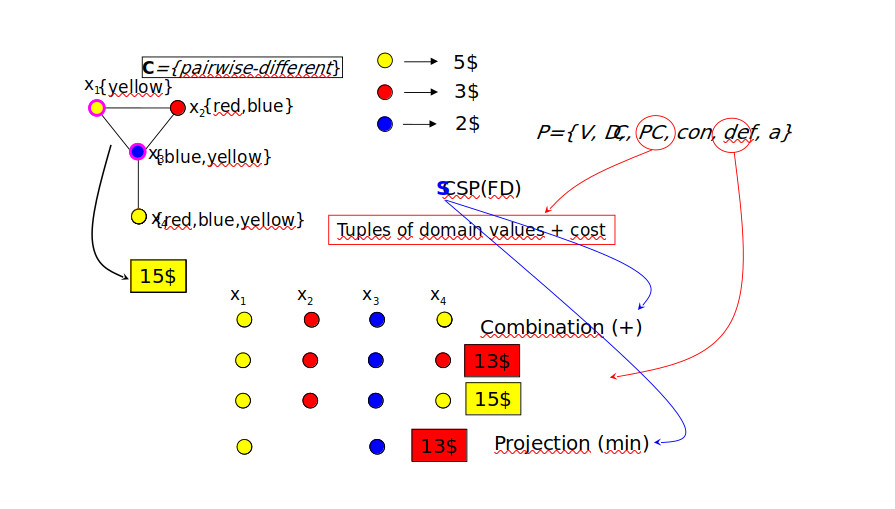
\includegraphics[width=14cm, keepaspectratio]{capitoli/img/Cap4/scsp2.png}
    \caption{Esempio di SCSP su grafo.}
\end{figure}

Partiamo riprendendo la definizione di un CSP, esso è definito come
$P=\{V,D,C,PC,con,def,a\}$ i quali indicano:
\begin{itemize}
    \item V $=$ insieme delle variabili;
    \item D $=$ insieme dei domini associati alle variabili;
    \item C $=$ insieme di vincoli, definito come l'associazione
          variabile-vincolo ovvero quali variabili sono coinvolte in quale vincolo;
    \item PC $=$ sono i vincoli primitivi e variano in base al vincolo e al
          dominio. A seconda del tipo di vincolo che possiamo avere i primitivi
          possono essere diversi, esempio se lavoro sugli interi esso conterrà
          vincoli con gli operatori $<,>,=$. \\Sostanzialmente esso indica i
          tipi di vincoli che posso usare se lavoro su un dominio specifico.
          Inoltre indicano se il vincolo è implicito (tutti i colori diversi) o
          esplicito (valgono le coppie $<r,g,b>, <g,r,b>, \ldots$).
    \item con $=$ funzione che definisce quali variabili sono coinvolte in quale
          vincolo, essa dato un vincolo restituisce le variabili che sono connesse a
          questo;
    \item def $=$ funzione che indica quali sono i valori del dominio possibili
          per una specifica variabile. In un SCSP questa funzione oltre a dire i
          valori possibili per una variabile deve indicare anche il costo associato a
          quei valori, nell'esempio in Figura 4.1 se passiamo in input alla funzione
          def la variabile $x_1$ essa ci ritornerà come valori possibile il colore giallo
          con costo 5. Questa è la differenza con la funzione def di un problema CSP.
    \item a $=$ sottoinsieme di V contenente tutte le variabili interessate
          nella soluzione del SCSP, ad esempio nel caso del grafo abbiamo che le
          variabili che ci interessano per la soluzione ottimale sono solo $x_1$ e
          $x_3$, non tutte quante.
\end{itemize}
Nell'esempio in Figura 4.1 i vincoli binari sono hard, perché la soluzione
richiede per forza che i nodi collegati abbiamo colori diversi sennò si violano
i vincoli, mentre i vincoli unari (quelli del costo sul colore) sono soft. Nel
caso di un CSP quando utilizziamo un algoritmo di ricerca per trovare una
soluzione esso si può fermare alla prima soluzione che trova oppure, se
richiesto, le cerca tutte quante. Nel caso di SCSP siamo costretti a trovare
tutte le possibili soluzioni in modo da scegliere la migliore. Normalmente si
utilizzano due operazioni per trovare la soluzione ottimale in un SCSP:

\begin{itemize}
    \item \textbf{Operatore di Combinazione($\times$):} dove metto insieme tutti gli
          assegnamenti, combinando i vincoli, quindi si calcola anche il costo totale
          ad esempio con l'operazione di somma;
    \item \textbf{Operatore di Proiezione ($+$):} operazione di scelta della
          soluzione migliore data dalla combinazione in base al minimo o al massimo
          del costo.
\end{itemize}

\section{Semiring}
Un semiring è una quintupla:
\begin{center}
    $<A, +, \times, 0, 1>$
\end{center}
\begin{itemize}
    \item \textbf{A:} \textit{l'insieme degli elementi} che mi rappresentano i costi
          (dominio dei costi). Esso può essere l'insieme dei reali oppure un
          intervallo specifico (ad esempio $[0,1]$)
    \item $+$: \textit{operatore di proiezione}, usato per fare la scelta fra le
          soluzioni trovate dalla combinazione, può essere il minimo o massimo.
          Possiamo definire alcune proprietà:
          \begin{itemize}
              \item \textbf{idempotente:} se faccio $a+a$ dove l'operatore $+$ è il
                    minimo il risultato è sempre a, quindi quando un operatore è
                    idempotente è possibile definire un ordinamento ovvero
                    \begin{center}
                        $a \leq b$ dove b è meglio di a $\Longleftrightarrow$
                        $a + b = b$
                    \end{center}
          \end{itemize}
    \item $\times$: \textit{operatore di combinazione}, utilizzato per combinare i
          vincoli, può essere somma,moltiplicazione etc... dipende dal problema.
          Possiamo definire alcune proprietà:
          \begin{itemize}
              \item \textbf{commutativa:} si considera il set di vincoli invece
                    delle tuple.
          \end{itemize}
    \item \textbf{0:} rappresenta il valore minimo (peggiore) dell'insieme A,
          ovvero il bottom sotto il quale non si può andare, per l'intervallo $[0,1]$
          è 0;
    \item \textbf{1:} rappresenta il valore massimo (migliore) di A, il top, per
          l'intervallo $[0,1]$ è 1.
\end{itemize}
Tutti questi che abbiamo visto sono simboli quindi quando si utilizza
l'operatore $+$ non ci si riferisce alla somma ma ad un operatore per la
proiezione che potrebbe essere $min, max, \text{OR}, \ldots$

\subsection{Tipi di Semiring}
\begin{itemize}
    \item \textbf{Probabilistic:} $<[0, 1], \max, \times, 0, 1>$ si massimizza
          la probabilità,
    \item \textbf{Weighted:} $<R^+, \min, +, +\infty, 0>$ si minimizza la somma
          dei costi,
    \item \textbf{Fuzzy:} $<[0,1], \max, \min, 0, 1>$,
    \item \textbf{Classical:} $<\{false,true\}, \ \lor(\text{OR}), \
              \land(\text{AND}), \ false, \ true>$.
\end{itemize}

\subsection{Esempi pratici SCSP: Domanda esame}
Il vincolo in mezzo è binario, se $a$ è compreso tra $x$ ed $y$.
\begin{center}
    $x \leq a \leq y$
\end{center}
A può assumere sia il valore di
\begin{enumerate}
    \item $x \rightarrow x = a$
    \item $y \rightarrow y = a$
\end{enumerate}

\subsubsection{Esempio con probabilistic}

\begin{figure}[H]
    \centering
    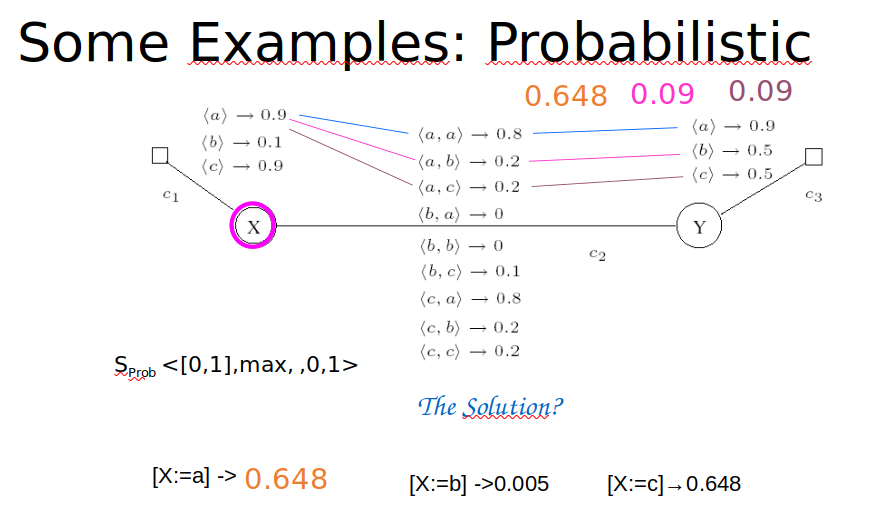
\includegraphics[width=12.5cm, keepaspectratio]{capitoli/img/Cap4/probabilistic2.png}
\end{figure}

\paragraph{Descrizione del semiring:} I valori possibili sono tra 0 ed 1,
l'operazione di proiezione è il Massimo; quella di combinazione è la
\textbf{moltiplicazione}; il minimo valore è 0; il massimo valore è 1. \\Ci
domandiamo: Quanto vale l'assegnamento X $=$ a?
\begin{enumerate}
    \item Dato che l'operazione $\times$ di combinazione è la moltiplicazione faccio:
          \begin{enumerate}
              \item $0.9*0.8*0.9 = 0.648$
              \item $0.9*0.2*0.5 = 0.09$
              \item $0.9*0.2*0.5 = 0.09$
          \end{enumerate}
          %% TODO: sta frase boh
          Per poter inserire 0.648 in $x = a$ dovrei dividere per 0.8 i 3 valori
          su $c_2$ e 0.9 i tre valori su $c_3$ (secondo me).
    \item Dato che l'operazione $+$ di proiezione in questo caso è $\max$ prendo il
          massimo di tutti gli elementi trovati e quella sarà la soluzione di
          quando ad X assegno a. Facendo lo stesso ragionamento si calcolano
          tutte le restanti soluzioni.
\end{enumerate}

\subsubsection{Esempio con Fuzzy}
\begin{figure}[H]
    \centering
    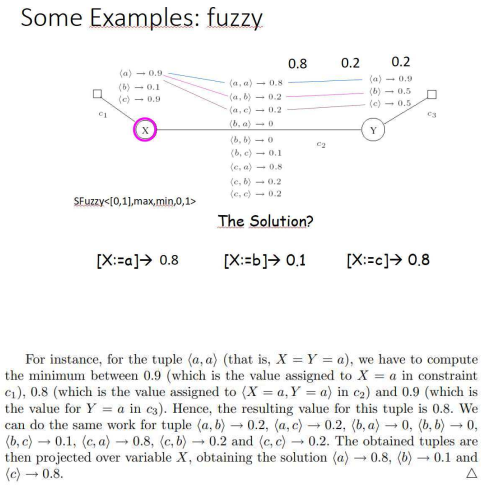
\includegraphics[width=12.5cm, keepaspectratio]{capitoli/img/Cap4/fuzzy.png}
\end{figure}

\paragraph{Teorema dell'Estensività: }
\begin{center}
    \textit{L'aggiunta di vincoli è monotona, peggiora la soluzione}
\end{center}
Questo significa che più aggiungo vincoli e più la soluzione peggiora, più tolgo
vincoli più la soluzione mi migliora. Questo perché più vincoliamo il problema e
meno possibilità abbiamo, meno lo vincoliamo e più sono le possibilità.

\subsubsection{Esempio di aggiunta vincolo (quindi peggioro)}

\begin{figure}[H]
    \centering
    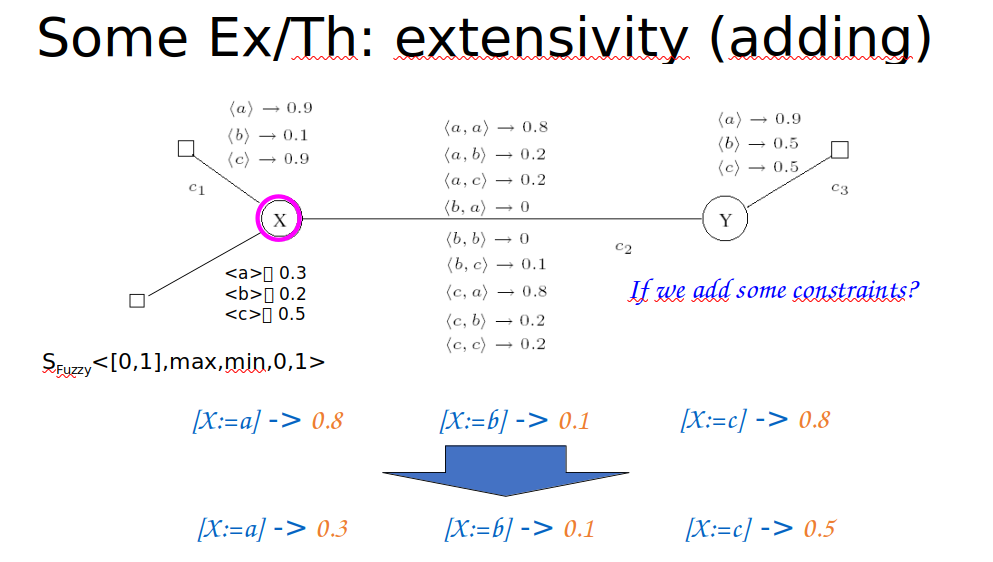
\includegraphics[width=12.5cm, keepaspectratio]{capitoli/img/Cap4/worst2.png}
\end{figure}

\subsubsection{Esempio di rimozione vincolo (quindi miglioro)}
\begin{figure}[H]
    \centering
    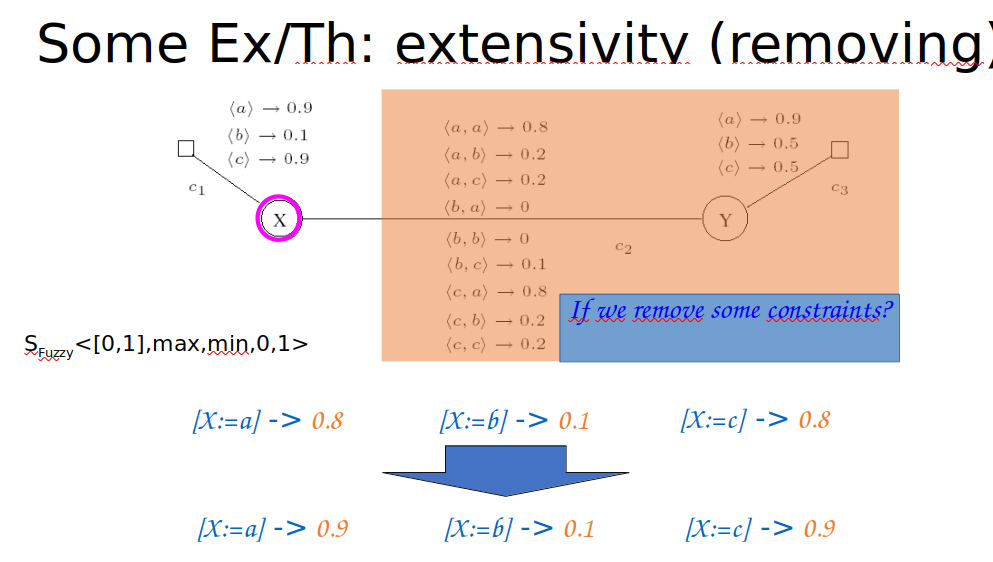
\includegraphics[width=12.5cm, keepaspectratio]{capitoli/img/Cap4/better2.png}
\end{figure}

\section{Local Consistency nei Soft CSP}
Fare Local consistency nel caso di CSP Soft non significa eliminare dei valori
dal dominio, ma significa ridurre (ottimizzare) il valore del semiring associato
a quella variabile in maniera tale da fare in modo che questo valore si avvicini
il più possibile a quello della soluzione finale.

\begin{center}
    \textit{Posso applicare Arc Consistency in un SCSP \textbf{solo} se l'operatore $\times$ è
        \textbf{idempotente}.}
\end{center}

Per esempio, non potremmo applicare Arc Consistency se come operatore $\times$
utilizzassimo la somma, ma potremmo farlo se usassimo $\min$.

\begin{center}
    $1 \times 1 = 2$ se $\times = somma$
\end{center}
\begin{center}
    $1 \times 1 = 1$ se $\times = minimo$
\end{center}

% \textbf{Teorema dell'estensività} Se tolgo dei vincoli da un problema SCSP, la
% soluzione migliora perché si moltiplica di meno (meno calcoli da fare),se li
% aggiungo la soluzione peggiora. Togliere vincoli vuol dire rilassare il
% problema. Se l'operatore x è idempotente allora possiamo applicare arc
% consistency, un esempio di operatore idempotente è il minimo se facciamo
% \begin{center}
%     $1 \times 1 = 2$ dove $×\times = somma$
% \end{center}
% \begin{center}
%     $1 \times 1 = 1$ se $\times = minimo$
% \end{center}
\subsection{Esempio con CSP Soft:}
\begin{figure}[H]
    \centering
    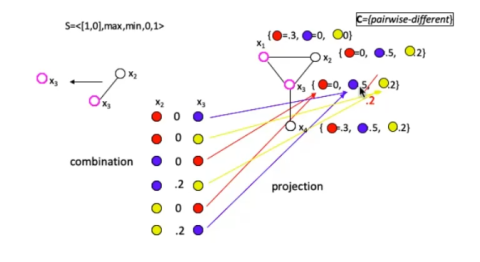
\includegraphics[width=14cm, keepaspectratio]{capitoli/img/Cap5/Local.png}
\end{figure}
\noindent In questo esempio sono presenti solo vincoli unari, ciò mi dice che
quando ad $x_1$  assegno rosso ha valore 0.3, quando blu o giallo ha valore
0; cosi per tutte le variabili. Siccome il valore 0 è il bottom del semiring,
dare 0 significa che non sono assegnamenti permessi, quindi li possiamo
direttamente eliminare.\\
\textbf{Ottimizzazione della soluzione su CSP Soft: } Voglio ridurre
(ottimizzare) il dominio della variabile $x_3$ , vediamo come fare con tutti i
passaggi:
\begin{enumerate}
    \item \textbf{Combinazione:} Prendo tutte le possibili tuple, gli assegno un
          valore e poi in base all'operatore di combinazione (che in questo caso
          è min) faccio la proiezione. \\Quindi parto cosi: Il minimo se $x_2$ è
          rosso e $x_3$ è blu è 0, perché è il minimo tra 0 e 0.5. \\Il minimo
          se $x_2$ è rosso e $x_3$ è giallo è 0, perché è il minimo tra 0 e 0.2.
          \\Continuo cosi per tutte le tuple. \\Non ho considerato le coppie di
          colore uguale perché c'era scritto $pairwise-different$.
    \item \textbf{Proiezione:} Tra tutti i risultati che genera la combinazione
          faccio la proiezione sulla variabile in questione, in questo caso $x_3$.
          Adesso: che valore ha $x_3$ quando ha valore rosso? Devo fare il massimo
          tra 0 e 0 che è 0 e tutto rimane invariato perché $x_3$ sul rosso ha
          comunque 0. Per $x_3$ $=$ blu il massimo è 0.2. Per $x_3$ $=$ giallo il
          massimo è comunque 0.2. L'unica modifica da apportare quindi è al blu di $x_3$
          che al posto di 0.5 ha valore 0.2.
\end{enumerate}
Nel caso \textbf{Crisp CSP} i valori vengono eliminati completamente dal
dominio. Nel caso \textbf{Soft CSP} ottimizzo il valore del semiring associato a
quell'assegnamento. Una volta ottimizzati tutti i valori si utilizzano tecniche
di \textbf{Branch And Bound}, che può essere applicato o all'inizio o durante la
ricerca, per trovare la soluzione.

\subsection{Esempio con Fuzzy}
\begin{figure}[htp]
    \centering
    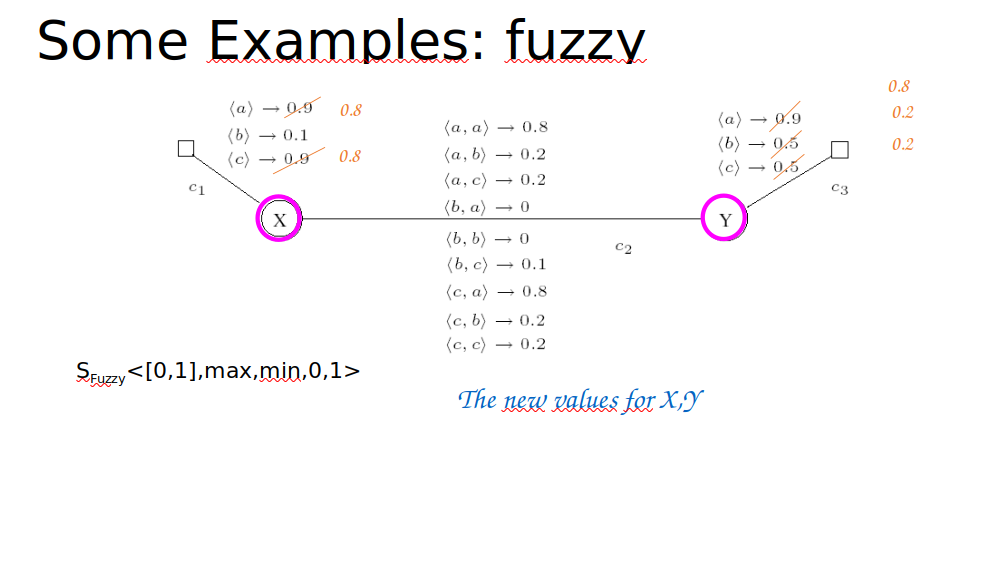
\includegraphics[width=14cm, keepaspectratio]{capitoli/img/Cap5/ffuzzy2.png}
\end{figure}
Consideriamo il vincolo unario $c_1$ sulla variabile X ed il vincolo binario $c_2$
sulle variabili X ed Y. Faccio $c_1$ $(x)$ $c_2$ proiettato $x(a)$:
\begin{enumerate}
    \item Combinazione (Min): $c_1$ combinato $c_2$ ($c_3$ non lo prendo in
          considerazione perché faccio $(x$):
          \begin{itemize}
              \item Quando vale $< a, a >?$ Faccio 0.9 min 0.8 $=$ 0.8
              \item Quando vale $< a, b >?$ Faccio 0.9 min 0.2 $=$ 0.2
              \item Quando vale $< a, c >?$ Faccio 0.9 min 0.2 $=$ 0.2
          \end{itemize}
          Facendo questo ho combinato i vincoli $c_1$ e $c_2$ . Per sapere poi quanto
          vale $c_1$ $(x)$ $c_2$ devo andare a proiettare su X.
    \item Proiezione (Max): Prendo il massimo tra 0.8, 0.2, 0.2. In conclusione,
          al posto di 0.9 su (a) posso scriverci 0.8.
\end{enumerate}
\textbf{Altra domanda sul fuzzy (assegnamento): } Quanto vale l'assegnamento
$x=a$, $y=b$? \\devo fare il minimo tra 0.9, 0.2 e 0.5 che sarebbe 0.2. \\(Non
applico la proiezione quindi non uso il massimo). \\Altra domanda: Applichiamo
local consistency per X $=$ a. \\Devo fare min(0.9, 0.8, 0.9) $=$ 0.8. \\Devo
fare min(0.9, 0.2, 0.5) $=$ 0.2. \\Devo fare min(0.9, 0.2, 0.5) $=$ 0.2. Se vado
a proiettare fa 0.8 perché prendo il massimo. Se io vado a calcolare la
soluzione, adesso vado a calcolare la soluzione di "quanto vale $x=a$ $y=b$"?
\\min tra 0.8, 0.2 e 0.2 = 0.2 che è come prima, la soluzione non è cambiata.
\textbf{Ho migliorato il bound ma non ho modificato la soluzione, è una cosa buona.}
\\Nell' esempio successivo (prossima sezione, sarebbe quello probabilistico) la
soluzione \textbf{viene modificata} a 0.72 e non più a 0.9 quindi non posso
accettarla, è proprio sbagliata.
\subsection{Idempotenza degli operatori}
Un operatore si dice idempotente se facendo:
\begin{center}
    $a$ $operazione$ $a$ mi restituisce sempre $a$.
\end{center}
L'idempotenza si può analizzare sia per gli operatori che si usano per la
Proiezione sia per quelli di Combinazione.\\
\begin{itemize}
    \item Idempotenza su \textbf{Combinazione}: Dipende strettamente dal
          semiring utilizzato:
          \begin{itemize}
              \item \textbf{Fuzzy:} Idempotente, perché il $minimo$ tra $a$ ed $a$ è
                    sempre $a$ (il minimo tra due valori uguali da sempre lo stesso
                    valore).
              \item \textbf{Probabilistic:} Non idempotente, perché $a * a$ non
                    fa esattamente $a$ (ad esempio $0.1 * 0.1 = 0.01$, la
                    moltiplicazione infatti non ha la proprietà di idempotenza).
              \item \textbf{Weighted:} Non idempotente, perché  $a + a$ non fa
                    esattamente $a$.
              \item \textbf{Classic:} Idempotente, infatti $a \text{ AND } a = a$
          \end{itemize}
    \item Idempotenza su \textbf{Proiezione:} Tutti gli operatori sono
          idempotenti e questo segue dalla definizione stessa di c-semiring (definisco
          l'ordinamento quando effettuo la proiezione).
\end{itemize}
La distinzione tra operatore idempotente e non idempotente è importante perché
gli algoritmi di consistenza locale solo nel caso in cui la combinazione fosse
idempotente \textbf{mantengono le soluzioni del problema}. Qualora facessi
arc-consistency su semiring che non ammettono operazioni idempotenti la
soluzione che si genera è proprio \textbf{sbagliata}, e non può essere
accettata.
\vspace{1cm}

\noindent \textbf{Vediamo un esempio in cui applicare arc-consistency va a
    modificare la soluzione finale del problema} (e quindi non è accettabile):
\begin{figure}[htp]
    \centering
    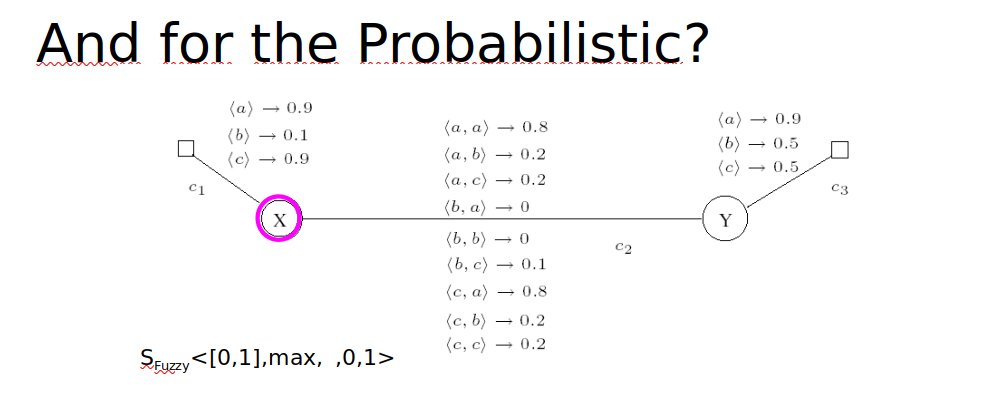
\includegraphics[width=14cm, keepaspectratio]{capitoli/img/Cap5/probabilistc2.png}
\end{figure}
\\
\textbf{Domanda:} Quanto vale l'assegnamento $x = a$, $y = b$ su questo
problema? \\devo moltiplicare 0.9, che sarebbe $x=a$, per $<x = a, y = b>$ che
sarebbe 0.2 per $y = b$ che sarebbe 0.5. Il risultato è 0.09. \\Domanda: Quanto
vale $c_1$ $c_2$ proiettato $x$ (su $a$)? devo fare la combinazione:
\begin{itemize}
    \item 0.9 $*$ 0.8 $=$ 0.72
    \item 0.9 $*$ 0.2 $=$ 0.18
    \item 0.9 $*$ 0.2 $=$ 0.18
\end{itemize}
Poi prendo il Massimo (proiezione) che sarebbe 0.72 e questo valore mi va al
posto di 0.9. Il problema però è che ho cambiato la soluzione finale, perché la
proiezione mi ritorna proprio il 0.72 che è un valore errato data la non
idempotenza della moltiplicazione (è proprio una soluzione sbagliata).\\

L'operazione di local consistency nei CSP Crisp quindi classici è
importante perché mantiene la soluzione del problema riducendo gli elementi del
dominio e non modificando le soluzioni.\\

Nel caso Soft invece, la soluzione non viene modificata solamente se
l'operazione di combinazione è idempotente. Nel caso in cui non lo fosse si
andrebbero a modificare le soluzioni stesse del problema, e quest'ultime non
sarebbero accettabili perché sbagliate.

\subsection{Altro esempio con vincolo \texorpdfstring{$c_3$}{c3}}
\begin{figure}[htp]
    \centering
    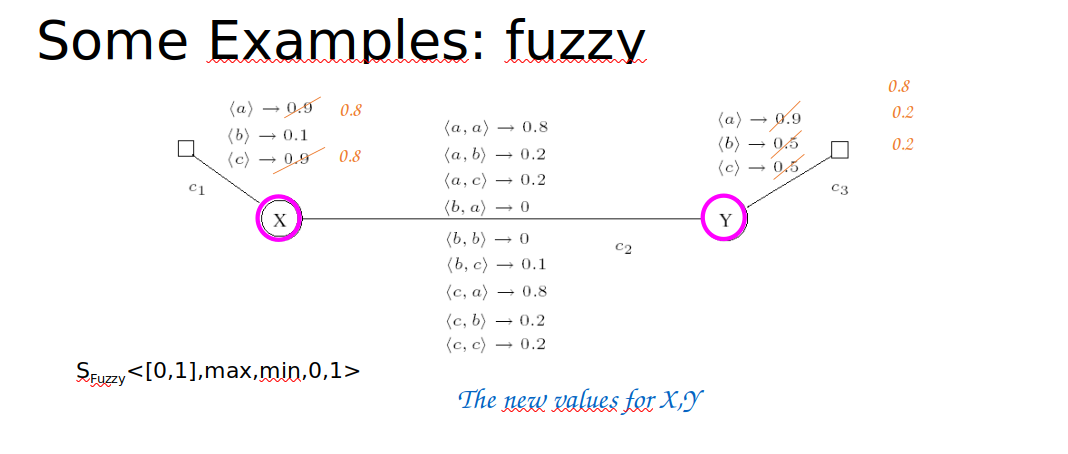
\includegraphics[width=14cm, keepaspectratio]{capitoli/img/Cap5/FUZZY2.png}
\end{figure}
I nuovi valori per il vincolo $c_3$ sono ottenuti analizzando prima $y = a$ e
quindi poi si analizza $<a, a>$ e poi $x = a$. Poi $y = b$ e quindi poi $<b, b>$ e
poi $x = b$. Utilizzando la combinazione e poi la proiezione i valori tornano
quelli.
\subsection{Semiring con operazioni non idempotenti}
% \subsubsection{Divisione}
Vogliamo ottimizzare i CSP Soft anche se la loro operazione di combinazione non
è idempotente.
\begin{figure}[htp]
    \centering
    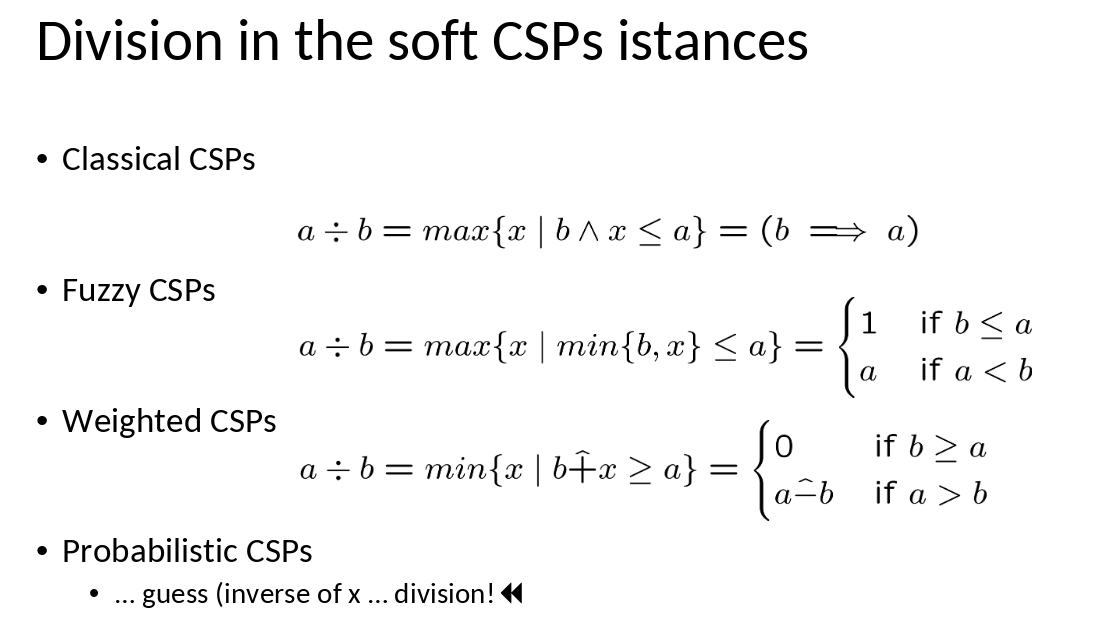
\includegraphics[width=13cm, keepaspectratio]{capitoli/img/Cap5/divisione.png}
\end{figure}
\\L'operatore che utilizzeremo è l'opposto dell'operatore di combinazione ed è
chiamato "\textit{Diviso}": $\div$. Analizziamo la riga del Fuzzy:
\begin{itemize}
    \item Prima versione: L'operazione inversa del minimo, indicata con
          l'operatore $\div$ è max. Supponiamo che l'elemento $x$ sia tale che
          $b * x = a$, la domanda è: Quanto fa $a \div b$? Fa quell'elemento $x$
          tale che il minimo tra $b$ ed $x$ è minore uguale di $a$. Devo quindi in
          qualche modo andarmi a trovare gli inversi degli operatori visti
          prima.
    \item  Seconda versione: Quando fa $a \div b$? (si legge "\textit{$a$ Diviso $b$}"). Fa il
          numero più grande $x$ tale che il minimo tra $b$ ed $x$ è più piccolo di $a$
\end{itemize}
Analizziamo la riga del \textbf{Weighted:}\\
Quanto fa $a \div b$? Fa il più
piccolo (min) elemento $x$ tale per cui $b + x$ fa $a$. Questo però lo possiamo fare
solo se $a$ è maggiore di $b$ (altrimenti si prenderebbero in considerazioni valori
non consoni tipo negativi) e se $b$ è maggiore uguale di $a$ si da come risultato 0.\\
\newpage

\textbf{Esempio probabilistico:}

\begin{figure}[H]
    \centering
    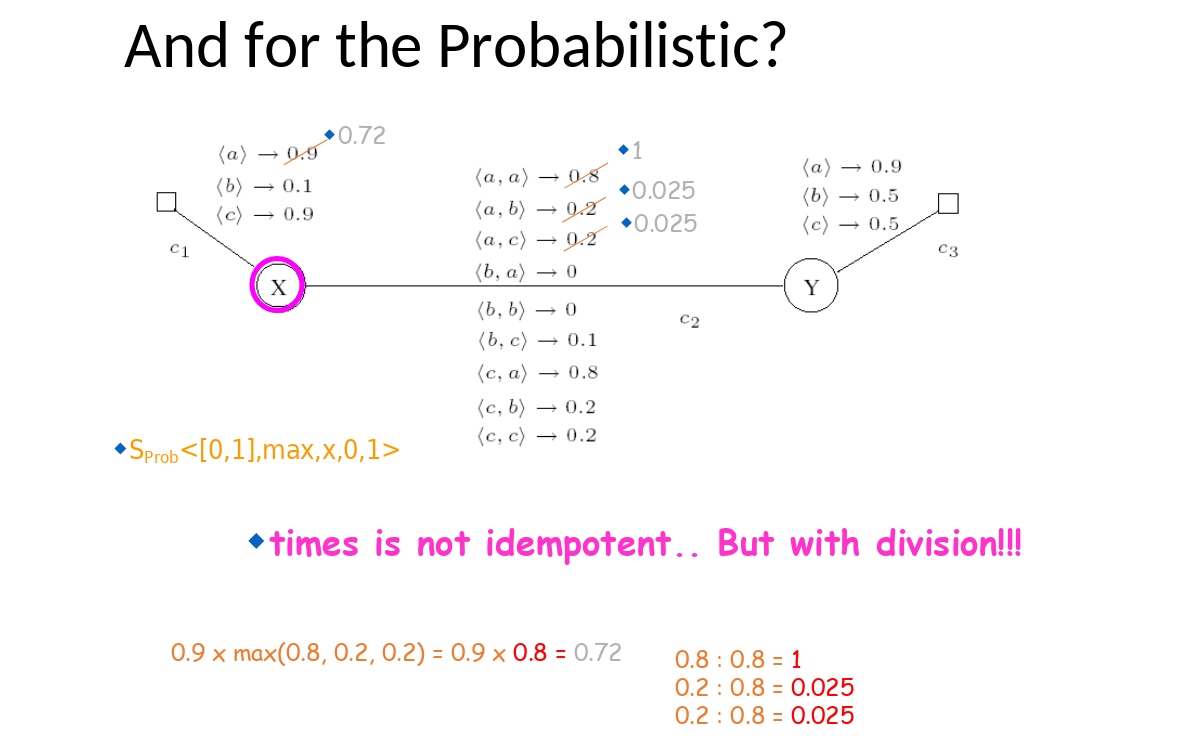
\includegraphics[width=14cm, keepaspectratio]{capitoli/img/Cap5/probabilisticmeglio.png}
    % PROBLEMA FOTO
\end{figure}

Come faccio ad ottimizzare il CSP in maniera tale da mantenere le soluzioni?
\\Inizio in maniera identica al precedente metodo:
\begin{itemize}
    \item Combinazione
          \begin{enumerate}
              \item 0.9 * 0.8 = 0.72
              \item 0.9 * 0.2 = 0.18
              \item 0.9 * 0.2 = 0.18
          \end{enumerate}
    \item Proiezione: Max = 0.72
\end{itemize}
\noindent Fatto questo devo \textbf{dividere per il massimo valore tra tutti
    quelli utilizzati:}
\begin{center}
    $max$(0.8, 0.2, 0.2) = 0.8
\end{center}
Ora divido per 0.8 tutti i valori nel vincolo $c_2$ cosi da ottenere i valori in
figura. Dato che ho ottimizzato il valore di (a) e cambiato i valori
interessati, la soluzione rimane invariata, quindi anche su semiring non
idempotenti si può fare arc-consistency grazie all'operatore di \textit{"Divisione"}
($\div$).

\paragraph{Importante:} in questo caso abbiamo utilizzato la
\textit{divisione} perché era l'operazione inversa della \textit{moltiplicazione} (che è
l'operatore di combinazione utilizzato nei CSP probabilistici). Se però
l'operazione di combinazione fosse stata la \textit{somma} (e quindi CSP Weighted)
l'operazione $\div$ sarebbe stata la \textit{sottrazione}.

